\subsection{Adaptive Quadrature}
    Romberg may achieve arbitrary accuracy but is not very efficient (function evaluations). Irregular function may waste evaluations in flat regions.
    
    \begin{center}
        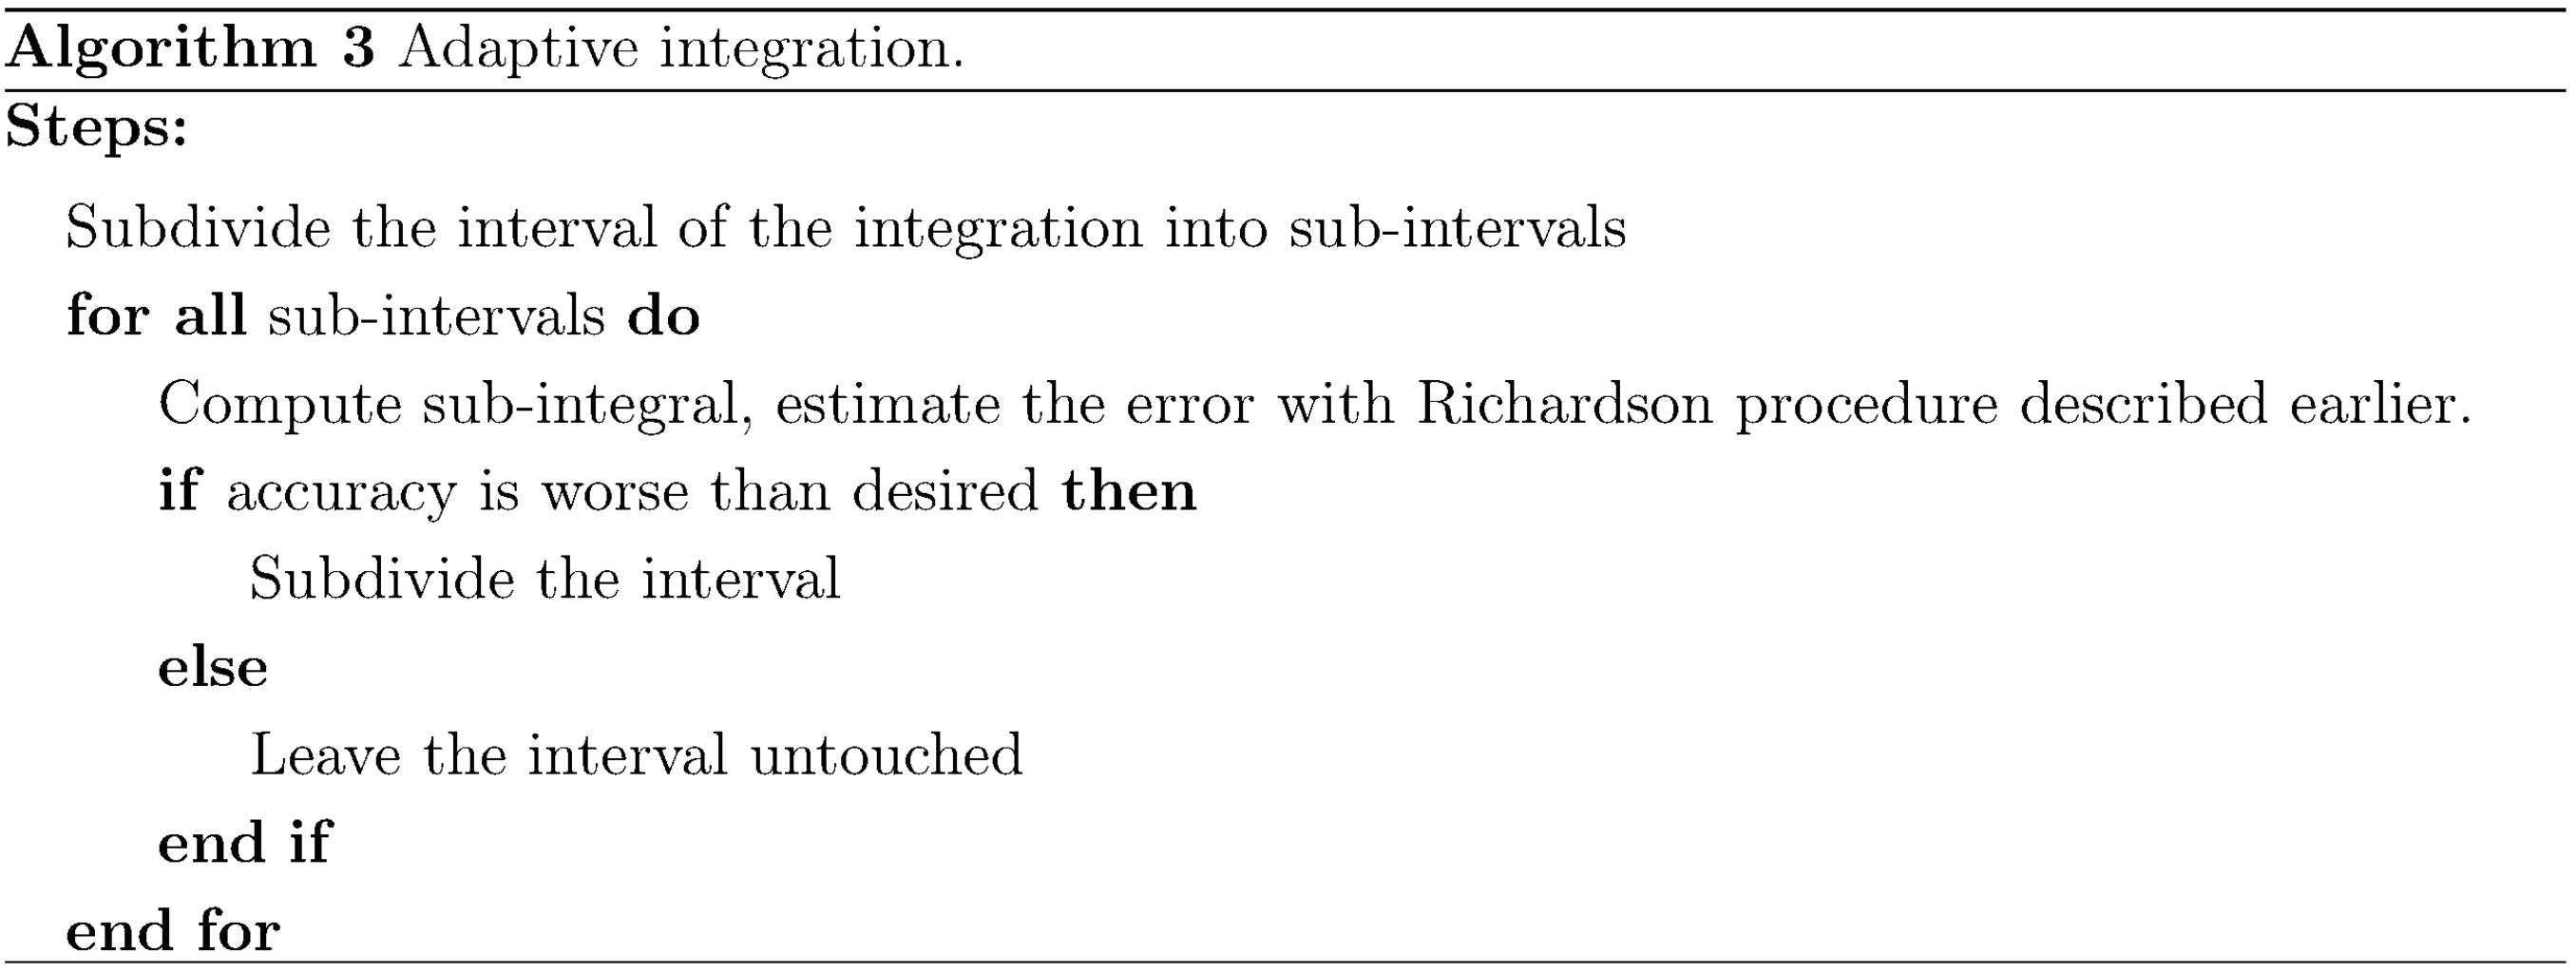
\includegraphics[width = \linewidth]{images/04/adaptive_quad.pdf}
    \end{center}
    
\subsection{Gauss Quadrature}
   We adapt the weights and abscissas of our quadrature rule to obtain better accuracy.
    
    \subsubsection{Two-Point Gauss Quadrature}
        The two point Gauss quadrature rule approximates $I$ using
        \begin{equation*}
            I = \int_a^b f(x)dx \approx c_1 f(x_1) + c_2 f(x_2)
        \end{equation*}
        where $c_1, \,c_2, \, x_1$ and $x_2$ are unknowns. They are evaluated by requiring an exact fit for an arbitrary third degree polynomial. Solving the nonlinear system of equations yields the two-point Gauss Quadrature rule:
        
        \begin{equation*}
            \colorboxed{red}{
            \begin{aligned}
            I \approx \frac{b-a}{2}\cdot f \left[\left(\frac{b-a}{2}\right)\left(\frac{-1}{\sqrt{3}}\right) + \frac{b+a}{2}\right]\\ +  \frac{b-a}{2}\cdot f\left[ \left(\frac{b-a}{2}\right)\left(\frac{1}{\sqrt{3}}\right) + \frac{b+a}{2}\right]
            \end{aligned}
            }
        \end{equation*}
    \subsubsection{\textit{n}-Point Gauss Quadrature}
        Goal: integrate $\int_a^b f(x)dx$.
        \begin{itemize}
            \item First we need to change the area of integration from $(a,b)$ with variable $\xi$ to $(-1,1)$ with variable $x$.
                \begin{equation*}
                    \colorboxed{red}{
                    z = \frac{2x - (a+b)}{b-a}
                    }
                \end{equation*}
                $I = \int_{-1}^1\frac{b-a}{2}f\left(\frac{b-a}{2}(z - 1) +b\right)dz$
            \item The integration points $z_i$ and the corresponding weights $w_i$ can be read from a table.
            
            \item the Integral is then evaluated using
            \begin{equation*}
            \colorboxed{red}{
                I \approx \frac{b-a}{2}\sum_{i=1}^n w_i f\left(\frac{b-a}{2}(z_i - 1) +b\right)
                }
            \end{equation*}
            
            \item Error with $n$ abscissas:
            \begin{equation*}
            \colorboxed{red}{
                \varepsilon = \frac{2^{2n+1}(n!)^4}{(2n+1)(2n!)^3}f^{(2n)}(\xi)
                }
            \end{equation*}
        \end{itemize}
        Gauss Quadrature gives the best accuracy, in the sense of correctly integrating polynomials of highest possible order for a given number of function evaluations. The Abscissas vary from order to order resulting in new evaluations of the abscissas from scratch if the accuracy of the Quadrature is to be improved.
        
        The abscissas are the zeros of the Legendre polynomial of degree $n$.
        
       